\section{Задача 2.4}
\subsection{Задание:}
Проверить тождество $ x^4 + 4 = (x - 1 - i)(x - 1 + i)(x + 1 + i)(x + 1 - i) $
\subsection{Решение:}
Преобразуем выражение:
\\[1em]
$
	(x - 1 - i)(x - 1 + i) \cdot (x + 1 + i)(x + 1 - i)
	=
	((x - 1)^2 - i^2) \cdot ((x + 1)^2 - i^2)
	=
	\\
	=
	((x - 1)^2 + 1) \cdot ((x + 1)^2 + 1)
	=
	(x^2 - 2x + 1 + 1) \cdot (x^2 + 2x + 1 + 1)
	=
	\\
	=
	(x^4 + 2x^3 + 2x^2 - 2x^3 - 4x^2 - 4x + 2x^2 + 4x + 4)
	=
	x^4 + 4
$
\\
Тождество верно.
\subsection{Проведём компьютерную проверку в среде Wolfram Mathematica:}
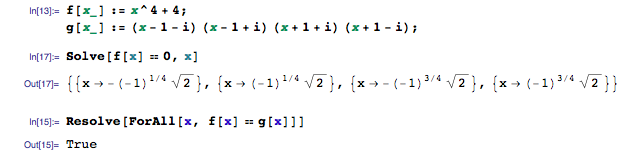
\includegraphics[scale=0.6]{task/2_04/screen1.png}
\subsection{Вывод:}
Проверка в компьютерной среде подтвердила верность тождества.
